\documentclass[aspectratio=169]{beamer}
\usepackage[utf8]{inputenc}

\usetheme{Madrid}
\usefonttheme[onlymath]{serif}

\AtBeginSection[]{
  \begin{frame}
  \vfill
  \centering
  \begin{beamercolorbox}[sep=8pt,center,shadow=true,rounded=true]{title}
    \usebeamerfont{title}\insertsectionhead\par%
  \end{beamercolorbox}
  \vfill
  \end{frame}
}

\usepackage{amsmath}
\usepackage{amssymb}
\usepackage{bm}

\renewcommand{\Vec}[1]{\bm{#1}}
\newcommand{\Mat}[1]{\mathbf{#1}}
\newcommand{\Tns}[1]{\mathcal{#1}}

\newcommand{\D}{\,\mathrm{d}}

\newcommand{\Ord}{\mathcal{O}}

\newcommand{\RR}{\mathbb{R}}

\usepackage{algpseudocode}

\usepackage{graphicx}
\usepackage{tikz}
\usetikzlibrary{arrows.meta,calc}

\title{Tensor Train Decomposition}
\author[Saibal De]{Saibal De \\ \texttt{saibalde@umich.edu}}
\date{October 29, 2020}

\begin{document}

\begin{frame}
    \titlepage
\end{frame}

\section{Recap}

\begin{frame}{Roadmap}
  \begin{itemize}
    \item
      Efficient matrix-vector multiplication is essential for fast algorithms
    \item
      FFT, FGT, FMM exploit low-rank structure of kernel matrices
    \item
      We can construct tensors using hierarchical domain decomposition
    \item
      {\color{red} Tensors constructed out of kernel matrices inherit low-rank
      structures}
    \item
      Tensor-train (TT) decomposition can capture low-rank structures very well
      \begin{itemize}
        \item
          Analytical solutions in rare cases
        \item
          TT-SVD for medium-sized tensors
        \item
          {\color{red} TT-cross for larger tensors}
      \end{itemize}
    \item
      Linear algebra operations are efficient in TT format
  \end{itemize}
\end{frame}

\begin{frame}{Unfolding and Hierarchical Domain Decomposition: Vectors}
  \centering
  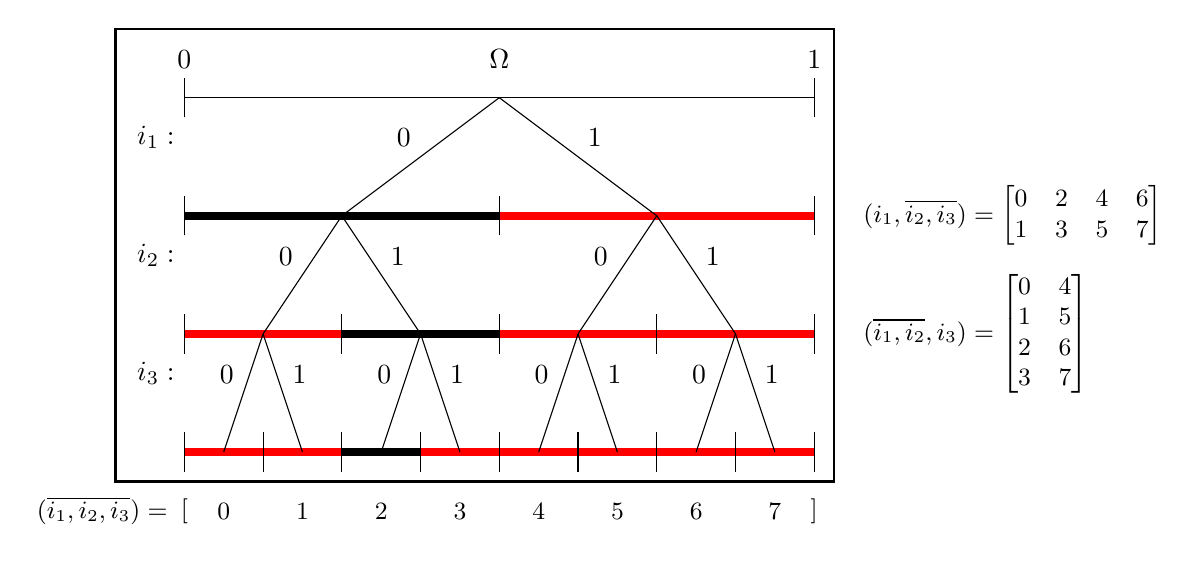
\begin{tikzpicture}[scale=0.25]
    % domain
    \draw ( 0, 18) -- (32, 18);
    \foreach \x in {0, 32} {
      \draw (\x, 17) -- (\x, 19);
    }
    \node [anchor=south] at ( 0, 19) {$0$};
    \node [anchor=south] at (16, 19) {$\Omega$};
    \node [anchor=south] at (32, 19) {$1$};

    % level 1
    \draw [line width=1mm, red] ( 0, 12) -- (32, 12);
    \foreach \x in {0, 16, 32} {
      \draw (\x, 11) -- (\x, 13);
    }
    \draw [line width=1mm] ( 0, 12) -- (16, 12);

    % level 2
    \draw [line width=1mm, red] ( 0,  6) -- (32,  6);
    \foreach \x in {0, 8, ..., 32} {
      \draw (\x,  5) -- (\x,  7);
    }
    \draw [line width=1mm] ( 8,  6) -- (16,  6);

    % level 3
    \draw [line width=1mm, red] ( 0,  0) -- (32,  0);
    \foreach \x in {0, 4, ..., 32} {
      \draw (\x,  -1) -- (\x,  1);
    }
    \draw [line width=1mm] ( 8,  0) -- (12,  0);

    % tree
    \draw (16, 18) -- node [anchor=south east] {$0$} ( 8, 12);
    \draw (16, 18) -- node [anchor=south west] {$1$} (24, 12);

    \draw ( 8, 12) -- node [anchor=south east] {$0$} ( 4,  6);
    \draw ( 8, 12) -- node [anchor=south west] {$1$} (12,  6);
    \draw (24, 12) -- node [anchor=south east] {$0$} (20,  6);
    \draw (24, 12) -- node [anchor=south west] {$1$} (28,  6);

    \draw ( 4,  6) -- node [anchor=south east] {$0$} ( 2,  0);
    \draw ( 4,  6) -- node [anchor=south west] {$1$} ( 6,  0);
    \draw (12,  6) -- node [anchor=south east] {$0$} (10,  0);
    \draw (12,  6) -- node [anchor=south west] {$1$} (14,  0);
    \draw (20,  6) -- node [anchor=south east] {$0$} (18,  0);
    \draw (20,  6) -- node [anchor=south west] {$1$} (22,  0);
    \draw (28,  6) -- node [anchor=south east] {$0$} (26,  0);
    \draw (28,  6) -- node [anchor=south west] {$1$} (30,  0);

    % tensor indices
    \node [anchor=east] at (0, 16) {$i_1:$};
    \node [anchor=east] at (0, 10) {$i_2:$};
    \node [anchor=east] at (0,  4) {$i_3:$};

    % boundary
    \draw [thick] (-3.5, -1.5) rectangle (33, 21.5);

    % vectorization
    \node [anchor=east] at (0, -3) {\small $(\overline{i_1, i_2, i_3}) =
      \null$};

    \node at ( 0,  -3) {\small $[$};
    \node at ( 2,  -3) {\small $0$};
    \node at ( 6,  -3) {\small $1$};
    \node at (10,  -3) {\small $2$};
    \node at (14,  -3) {\small $3$};
    \node at (18,  -3) {\small $4$};
    \node at (22,  -3) {\small $5$};
    \node at (26,  -3) {\small $6$};
    \node at (30,  -3) {\small $7$};
    \node at (32,  -3) {\small $]$};

    % unfoldings
    \node [anchor=west] at (34, 12) {\small $(i_1, \overline{i_2, i_3}) =
      \begin{bmatrix}
        0 & 2 & 4 & 6 \\
        1 & 3 & 5 & 7
      \end{bmatrix}
    $};

    \node [anchor=west] at (34, 6) {\small $(\overline{i_1, i_2}, i_3) =
      \begin{bmatrix}
        0 & 4 \\
        1 & 5 \\
        2 & 6 \\
        3 & 7
      \end{bmatrix}
    $};
  \end{tikzpicture}
\end{frame}

\begin{frame}{Unfolding and Hierarchical Domain Decomposition: Matrices}
  \centering
  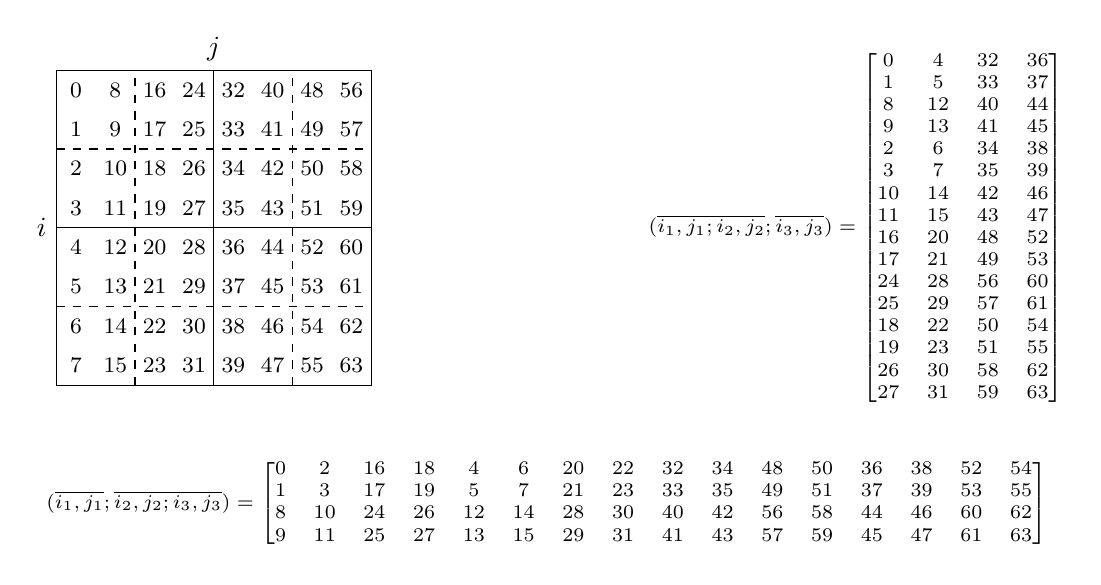
\begin{tikzpicture}[scale=0.5]
    \foreach \x in {0.5, 1.5, ..., 7.5} {
      \foreach \y in {0.5, 1.5, ..., 7.5} {
        \pgfmathsetmacro\z{int(8 * (\x - 0.5) + 7 - (\y - 0.5))}
        \node at (\x, \y) {\footnotesize ${\z}$};
      }
    }
    \draw (0, 0) rectangle (8, 8);
    \draw (0, 4) -- (8, 4);
    \draw (4, 0) -- (4, 8);
    \draw [dashed] (0, 2) -- (8, 2);
    \draw [dashed] (0, 6) -- (8, 6);
    \draw [dashed] (2, 0) -- (2, 8);
    \draw [dashed] (6, 0) -- (6, 8);
    \node [anchor=east] at (0, 4) {$i$};
    \node [anchor=south] at (4, 8) {$j$};

    \node [anchor=west] at (-0.5, -3) {\scriptsize $(\overline{i_1, j_1};
    \overline{i_2, j_2; i_3, j_3}) =
    \begin{bmatrix}
      \begin{matrix}
        0 &  2 & 16 & 18 &  4 &  6 & 20 & 22 \\
        1 &  3 & 17 & 19 &  5 &  7 & 21 & 23 \\
        8 & 10 & 24 & 26 & 12 & 14 & 28 & 30 \\
        9 & 11 & 25 & 27 & 13 & 15 & 29 & 31
      \end{matrix}
      &
      \begin{matrix}
        32 & 34 & 48 & 50 & 36 & 38 & 52 & 54 \\
        33 & 35 & 49 & 51 & 37 & 39 & 53 & 55 \\
        40 & 42 & 56 & 58 & 44 & 46 & 60 & 62 \\
        41 & 43 & 57 & 59 & 45 & 47 & 61 & 63
      \end{matrix}
    \end{bmatrix}$};

    \node [anchor=west] at (14.8, 4) {\scriptsize $(\overline{i_1, j_1; i_2,
    j_2}; \overline{i_3, j_3}) =
    \begin{bmatrix}
       0 &  4 & 32 & 36 \\
       1 &  5 & 33 & 37 \\
       8 & 12 & 40 & 44 \\
       9 & 13 & 41 & 45 \\
       2 &  6 & 34 & 38 \\
       3 &  7 & 35 & 39 \\
      10 & 14 & 42 & 46 \\
      11 & 15 & 43 & 47 \\
      16 & 20 & 48 & 52 \\
      17 & 21 & 49 & 53 \\
      24 & 28 & 56 & 60 \\
      25 & 29 & 57 & 61 \\
      18 & 22 & 50 & 54 \\
      19 & 23 & 51 & 55 \\
      26 & 30 & 58 & 62 \\
      27 & 31 & 59 & 63
    \end{bmatrix}$};
  \end{tikzpicture}
\end{frame}

\begin{frame}{Tensor-Train Format}
  \begin{itemize}
    \item
      Matrix form
      \begin{equation*}
        \Tns{X}(i_1, i_2, \ldots, i_d) = \underbrace{\Mat{X}_1(i_1)}_{r_0 \times
        r_1} \underbrace{\Mat{X}_2(i_2)}_{r_1 \times r_2} \cdots
        \underbrace{\Mat{X}_d(i_d)}_{r_{d - 1} \times r_d}, \quad r_0 = r_d = 1
      \end{equation*}
    \item
      Element form
      \begin{equation*}
        \Tns{X}(i_1, i_2, \ldots, i_d) = \sum_{\alpha_0 = 1}^{r_0}
        \sum_{\alpha_1 = 1}^{r_1} \cdots \sum_{\alpha_d = 1}^{r_d}
        \Tns{X}_1(\alpha_0, i_1, \alpha_1) \Tns{X}_2(\alpha_1, i_2, \alpha_2)
        \cdots \Tns{X}_d(\alpha_{d - 1}, i_d, \alpha_d)
      \end{equation*}
    \item
      Computational costs:
      \begin{itemize}
        \item
          Storage: $\Ord(d n r^2)$
        \item
          Single entry evaluation: $\Ord(d r^2)$
      \end{itemize}
  \end{itemize}
\end{frame}

\begin{frame}{Fast Operations in TT Format}
  \begin{itemize}
    \item
      Scalar multiplication: $\Tns{Y} = \alpha \Tns{X}$
      \begin{equation*}
        \Mat{Y}_1(i_1) = \alpha \Mat{X}_1(i_1), \quad \Mat{Y}_k(i_k) =
        \Mat{X}_k(i_k)
      \end{equation*}
    \item
      Vector addition: $\Tns{Z} = \Tns{X} + \Tns{Y}$
      \begin{equation*}
        \Mat{Z}_1(i_1) =
        \begin{bmatrix}
          \Mat{X}_1(i_1) & \Mat{Y}_1(i_1)
        \end{bmatrix},
        \quad \Mat{Z}_k(i_k) =
        \begin{bmatrix}
          \Mat{X}_k(i_k) & \\
                         & \Mat{Y}_k(i_k)
        \end{bmatrix},
        \quad \Mat{Z}_d(i_d) =
        \begin{bmatrix}
          \Mat{X}_d(i_d) \\
          \Mat{Y}_d(i_d)
        \end{bmatrix}
      \end{equation*}
    \item
      Dot product: $\langle \Tns{X}, \Tns{Y} \rangle = \texttt{sum}(\Tns{Z})$,
      $\Tns{Z} = \Tns{X} \circ \Tns{Y}$
      \begin{equation*}
        \Mat{Z}_k(i_k) = \Mat{X}_k(i_k) \otimes \Mat{Y}_k(i_k)
      \end{equation*}
  \end{itemize}
\end{frame}

\begin{frame}{TT-SVD}
  \begin{algorithmic}[1]
    \Require {$d$-dimensional tensor $\Tns{X} \in \RR^{n_1 \times \cdots \times
    n_d}$, relative accuracy $\epsilon$}
    \Ensure {TT cores $\Tns{Y}_1, \ldots, \Tns{Y}_d$ of tensor $\Tns{Y}$
    satisfying $\lVert \Tns{X} - \Tns{Y} \rVert_F \leq \epsilon \lVert \Tns{X}
    \rVert_F$}
    \Statex
    \State {Compute truncation parameter $\delta = \epsilon \lVert \Tns{X}
    \rVert_F / \sqrt{d - 1}$}
    \State {$r_0 = 1$}
    \State {$\Mat{C} = \texttt{reshape}(\Tns{X}, [r_0 n_1, n_2 \cdots n_d])$}
    \For {$k = 1, \ldots, d - 1$}
      \State {$\Mat{U}, \Mat{\Sigma}, \Mat{V} = \texttt{truncated-svd}(\Mat{C},
      \delta)$}
      \State {$r_k = \texttt{size}(\Mat{\Sigma}, 1)$}
      \State {$\Tns{Y}_k = \texttt{reshape}(\Mat{U}, [r_{k - 1}, n_k, r_k])$}
      \State {$\Mat{C} = \texttt{reshape}(\Mat{\Sigma} \Mat{V}^\top, [r_k n_{k +
      1}, n_{k + 2} \cdots n_d])$}
    \EndFor
    \State {$r_d = 1$}
    \State {$\Tns{Y}_d = \texttt{reshape}(\Mat{C}, [r_{d - 1}, n_d, r_d])$}
  \end{algorithmic}
\end{frame}

\section{Rounding}

\begin{frame}{Rank Inflation}
  \begin{itemize}
    \item
      Linear algebra operations in TT format often inflate TT ranks
    \item
      Consider TT decomposition $\Tns{X}(i_1, \ldots, i_d) = \Mat{X}_1(i_1)
      \cdots \Mat{X}_d(i_d)$
    \item
      The TT decomposition corresponding to $\Tns{Y} = \Tns{X} + \Tns{X}$ is
      \begin{equation*}
        \Mat{Y}_1(i_1) =
        \begin{bmatrix}
          \Mat{X}_1(i_1) & \Mat{X}_1(i_1)
        \end{bmatrix},
        \quad \Mat{Y}_k(i_k) =
        \begin{bmatrix}
          \Mat{X}_k(i_k) & \\
                         & \Mat{X}_k(i_k)
        \end{bmatrix},
        \quad \Mat{Y}_d(i_d) =
        \begin{bmatrix}
          \Mat{X}_d(i_d) \\
          \Mat{X}_d(i_d)
        \end{bmatrix}
      \end{equation*}
      with maximal rank $r_{\Tns{Y}} = 2 r_{\Tns{X}}$
    \item
      The TT decomposition corresondign to $\Tns{Z} = 2 \Tns{X}$ is
      \begin{equation*}
        \Mat{Z}_1(i_1) = 2 \Mat{X}_1(i_1), \quad \Mat{Z}_k(i_k) = \Mat{X}_k(i_k)
      \end{equation*}
      with maximal rank $r_{\Tns{Z}} = r_{\Tns{X}}$
  \end{itemize}
\end{frame}

\begin{frame}{TT-round}
  \begin{algorithmic}[1]
    \Require {$d$-dimensional tensor $\Tns{X}$ in TT format, relative accuracy
    $\epsilon$}
    \Ensure {TT cores $\Tns{Y}_1, \ldots, \Tns{Y}_d$ of tensor $\Tns{Y}$ with
    optimal ranks satisfying $\lVert \Tns{X} - \Tns{Y} \rVert_F \leq \epsilon
    \lVert \Tns{X} \rVert_F$}
    \Statex
    \State {Compute truncation parameter $\delta = \epsilon \lVert \Tns{X}
    \rVert_F / \sqrt{d - 1}$}
    \State {Let $\Tns{G}_1, \ldots, \Tns{G}_d$ be the cores of $\Tns{X}$}
    \For {$k = d, d - 1, \ldots, 2$}
      \State {Row-QR decomposition: $\Mat{G}_k^{(1)} = \Mat{R} \Mat{G}_k^{(1)}$}
      \State {$\Mat{G}_{k - 1}^{(2)} = \Mat{G}_{k - 1}^{(2)} \Mat{R}$}
    \EndFor
    \For {$k = 1, \ldots, d - 1$}
      \State {Truncated SVD: $\Mat{G}_k^{(2)} = \Mat{G}_k^{(2)} \Mat{\Sigma}
      \Mat{V}^\top + \Mat{E}$, $\lVert \Mat{E} \rVert_F \leq \delta$}
      \State {$\Mat{G}_{k + 1}^{(2)} = \Mat{\Sigma} \Mat{V}^\top \Mat{G}_{k +
      1}^{(2)}$}
    \EndFor
    \State {Let $\Tns{G}_1, \ldots, \Tns{G}_d$ be the cores of $\Tns{Y}$}
  \end{algorithmic}
\end{frame}

\section{Matrix Operations}

\begin{frame}{Matrix-Vector Multiplication}
  \begin{itemize}
    \item
      Matrix $\Tns{K}(i_1, j_1, \ldots, i_d, j_d) = \Mat{K}_1(i_1, j_1) \cdots
      \Mat{K}_d(i_d, j_d)$
    \item
      Vector $\Tns{X}(j_1, \ldots, j_d) = \Mat{X}_1(j_1) \cdots \Mat{X}_d(j_d)$
    \item
      Product
      \begin{equation*}
        \begin{split}
          \Tns{Y}(i_1, \ldots, i_d)
          &= \sum_{j_1, \ldots, j_d} \Tns{K}(i_1, j_1, \ldots, i_d, j_d)
          \Tns{X}(j_1, \ldots, j_d) \\
          &= \sum_{j_1, \ldots, j_d} [\Mat{K}_1(i_1, j_1) \cdots \Mat{K}_d(i_d,
          j_d)] \otimes [\Mat{X}_1(j_1) \cdots \Mat{X}_d(j_d)] \\
          &= \left(\sum_{j_1} \Mat{K}_1(i_1, j_1) \Mat{X}_1(j_1)\right) \cdots
          \left(\sum_{j_d} \Mat{K}_d(i_d, j_d) \Mat{X}_d(j_d)\right)
        \end{split}
      \end{equation*}
    \item
      Thus $\Mat{Y}_k(i_k) = \sum_{j_k} \Mat{K}_k(i_k, j_k) \otimes
      \Mat{X}_k(j_k)$
  \end{itemize}
\end{frame}

\begin{frame}{Matrix-Vector Multiplication}
  \begin{itemize}
    \item
      But what if the vector is not in TT format?
    \item
      Apply the cores one-by-one
      \begin{equation*}
        \begin{split}
          \Tns{Y}(i_1, \ldots, i_d)
          &= \sum_{j_1, \ldots, j_d} \Tns{K}(i_1, j_1, \ldots, i_d, j_d)
          \Tns{X}(j_1, \ldots, j_d) \\
          &= \sum_{j_1, \ldots, j_d} \Mat{K}_1(i_1, j_1) \cdots \Mat{K}_d(i_d,
          j_d) \Tns{X}(j_1, \ldots, j_d) \\
          &= \sum_{j_1} \Mat{K}_1(i_1, j_1) \cdots \sum_{j_d} \Mat{K}_d(i_d,
          j_d) \Tns{X}(j_1, \ldots, j_d)
        \end{split}
      \end{equation*}
  \end{itemize}
\end{frame}

\section{TT Interpolation}

\begin{frame}{Limitations of TT-SVD}
  \begin{itemize}
    \item
      TT-SVD operates by running SVD on the unfolding matrices
    \item
      Running SVD requires knowing {\color{red} all} matrix entries
    \item
      TT-SVD is suitable only for small/medium sized tensors
    \item
      There is nothing special about SVD!
  \end{itemize}
\end{frame}

\begin{frame}{Skeleton Decomposition}
  \begin{itemize}
    \item
      Skeleton decomposition: For a rank-$r$ matrix $\Mat{X} \in \RR^{m \times
      n}$ there exists a decomposition
      \begin{equation*}
        \Mat{X} = \Mat{X}(:, \mathcal{J}) \Mat{X}(\mathcal{I}, \mathcal{J})^{-1}
        \Mat{X}(\mathcal{I}, :)
      \end{equation*}
      where $\mathcal{I}$ and $\mathcal{J}$ are $r$ row and column indices such
      that $\Mat{X}(\mathcal{I}, \mathcal{J})$ is invertible
    \item
      We do not need to know all the entries of a matrix!
  \end{itemize}
\end{frame}

\begin{frame}{Interpolative Decomposition}
  \begin{itemize}
    \item
      Compute the TT decomposition from entry evaluation $\Tns{X}(i_1, \ldots,
      i_d)$
    \item
      Only evaluate the tensor at $\Ord(d n r^2)$ entries
    \item
      Several implementations:
      \begin{itemize}
        \item
          TT-cross
        \item
          TT-DMRG-cross
        \item
          TT-AMEn-cross
      \end{itemize}
  \end{itemize}
\end{frame}

\begin{frame}{Matrix Solve}
  \begin{itemize}
    \item
      Both $\Tns{K}(i_1, j_1, \ldots, i_d, j_d)$ and $\Tns{Y}(i_1, \ldots, i_d)$
      are in TT format
    \item
      DMRG-solve, AMEn-solve can compute the solution to
      \begin{equation*}
        \Tns{K} \Tns{X} = \Tns{Y}
      \end{equation*}
      in TT format
      \begin{itemize}
        \item
          Start from an initial guess $\Tns{X}_0$
        \item
          Iterate over the cores one-by-one, minimizing the error
          \begin{equation*}
            \lVert \Tns{K} \Tns{X} - \Tns{Y} \rVert_F^2 \to \min
          \end{equation*}
        \item
          Reduces to a small linear system with current core as unknown
      \end{itemize}
  \end{itemize}
\end{frame}

\section{Miscellaneous}

\begin{frame}{Code}
  \begin{itemize}
    \item
      Tensor Train codes by I.\ V.\ Oseledets:
      \begin{itemize}
        \item
          MATLAB: \texttt{https://github.com/oseledets/TT-Toolbox}
        \item
          Python: \texttt{https://github.com/oseledets/ttpy}
      \end{itemize}
    \item
      Class demo: \texttt{https://github.com/saibalde/math671-tt-lecture}
  \end{itemize}
\end{frame}

\begin{frame}{References}
  \begin{itemize}
    \item
      Ivan Oseledets (2011). \textit{Tensor-train decomposition.} SIAM Journal
      on Scientific Computing.
    \item
      Ivan Oseledets, Eugene Tyrtyshnikov and Nickolai Zamarashkin (2011).
      \textit{Tensor-train ranks for matrices and their inverses.} Computational
      Methods in Applied Mathematics.
    \item
      Ivan Oseledets and Eugene Tyrtyshnikov (2010). \textit{TT-cross
      approximation for multidimensional arrays.} Linear Algebra and its
      Applications.
    \item
      Ivan Oseledets (2011). \textit{DMRG approach to fast linear algebra in the
      TT-format.} Computational Methods in Applied Mathematics.
    \item
      Dmitry Savostyanov and Ivan Oseledets (2011). \textit{Fast adaptive
      interpolation of multi-dimensional arrays in tensor-train format.}
      International Workshop on Multidimensional Systems. IEEE.
    \item
      Sergey Dolgov and Dmitry Savostyanov (2014). \textit{Alternating minimal
      energy methods for linear systems in higher dimensions}. SIAM Journal on
      Scientific Computing.
  \end{itemize}
\end{frame}

\end{document}
